\documentclass[11pt,a4paper]{article}

% ── Packages ──────────────────────────────────────────────────────────────
\usepackage[utf8]{inputenc}
\usepackage[T1]{fontenc}
\usepackage{amsmath,amssymb}
\usepackage{graphicx}
\usepackage{booktabs}
\usepackage{hyperref}
\usepackage[margin=2.5cm]{geometry}
\usepackage{natbib}
\usepackage{xcolor}
% algorithm/algpseudocode not available; pseudocode via lstlisting
\usepackage{listings}
\usepackage{tikz}
\usetikzlibrary{trees,positioning,arrows.meta,shapes.geometric}
\usepackage{float}
\usepackage{caption}
\usepackage{subcaption}
\usepackage{enumitem}
\usepackage{microtype}
\usepackage{authblk}

% ── Listing style ─────────────────────────────────────────────────────────
\lstset{
  basicstyle=\ttfamily\small,
  keywordstyle=\color{blue!70!black}\bfseries,
  commentstyle=\color{green!50!black}\itshape,
  stringstyle=\color{red!60!black},
  numbers=left,
  numberstyle=\tiny\color{gray},
  numbersep=6pt,
  frame=single,
  framexleftmargin=2mm,
  breaklines=true,
  showstringspaces=false,
  captionpos=b,
  tabsize=4,
}

\lstdefinelanguage{yaml}{
  morekeywords={focal_species,chromosome_lengths,chromosomes,outgroups,inner,outer,
    name,alignment,output_dir,num_cpus,method,tree,backend,gpu_devices,evaluation,
    reference_dir,reference_pattern,vcf_dir,vcf_pattern,min_inner_freq,min_outer_freq,
    ml_model_path,ml_high_threshold,ml_low_threshold},
  sensitive=true,
  morecomment=[l]{\#},
  morestring=[b]",
  morestring=[b]',
}

% ── Title ─────────────────────────────────────────────────────────────────
\title{\textbf{ancify: A Config-Driven Pipeline for Ancestral Allele\\
Polarization Using Outgroup Alignments}}

\author[1]{Kevin Korfmann}
\affil[1]{Independent Researcher}

\date{\today}

% ══════════════════════════════════════════════════════════════════════════
\begin{document}
\maketitle

% ── Abstract ──────────────────────────────────────────────────────────────
\begin{abstract}
Determining the ancestral state of segregating alleles is a prerequisite for
constructing unfolded site frequency spectra, detecting natural selection, and
inferring demographic history. We present \textbf{ancify}, an open-source,
species-agnostic Python pipeline that infers per-position ancestral alleles
from pairwise net-AXT alignments with multiple outgroup species. The tool
implements three complementary inference methods: (i)~a two-tier inner/outer
outgroup voting scheme that guards against incomplete lineage sorting,
(ii)~Fitch parsimony on a user-supplied phylogenetic tree, and (iii)~a
LightGBM gradient-boosted classifier that learns substitution biases from
data. All methods produce FASTA output with case-encoded confidence levels.
An optional GPU-accelerated backend using PyTorch reduces genome-wide
processing time from approximately 12~hours to under 2~minutes for the
human genome. Validation against the Ensembl EPO 13-primate ancestral
reference yields $>$99.9\% agreement on human autosomes. ancify is
distributed under the MIT license and is available at
\url{https://github.com/kevinkorfmann/ancify}.
\end{abstract}

\vspace{0.5em}
\noindent\textbf{Keywords:}
ancestral allele, polarization, site frequency spectrum, outgroup alignment,
incomplete lineage sorting, Fitch parsimony, GPU acceleration, population genetics

% ══════════════════════════════════════════════════════════════════════════
\section{Introduction}
\label{sec:introduction}

Understanding the direction of evolutionary change at polymorphic sites is
fundamental to population genetics. The distinction between the \emph{ancestral}
allele---the state present in the most recent common ancestor of a sample---and
the \emph{derived} allele---the product of a more recent mutation---underlies
virtually all inference about demographic history, natural selection, and
mutational processes \citep{Kimura1983,Watterson1975}.

The \emph{site frequency spectrum} (SFS), the distribution of allele
frequencies across segregating sites in a population, is one of the most
widely used summary statistics in population genetics. In its
\emph{unfolded} (polarized) form, the SFS distinguishes rare derived alleles
from rare ancestral alleles, providing substantially more information than
the symmetric \emph{folded} SFS. Tools for demographic inference
\citep{Gutenkunst2009,Jouganous2017}, selection scans
\citep{Nielsen2005,Fay2000}, and mutation rate estimation
\citep{DeGiorgio2016} typically require or strongly benefit from the
unfolded SFS.

Ancestral state determination relies on the parsimony principle: if multiple
outgroup species carry the same allele at a site, the simplest explanation
is that this allele was present in the common ancestor, and the alternative
allele in the focal species arose by mutation. However, several complications
arise in practice:

\begin{enumerate}[leftmargin=2em]
    \item \textbf{Incomplete lineage sorting (ILS):} When ancestral
        populations were large and speciation events were temporally close,
        gene trees may disagree with the species tree at a non-trivial
        fraction of loci \citep{Degnan2009,Hobolth2011}. For the
        human--chimpanzee--gorilla clade, ILS affects approximately
        1--3\% of the genome \citep{Scally2012}.
    \item \textbf{Back mutations and convergent substitutions:} The
        outgroup may have undergone an independent mutation at the same
        site, masking the true ancestral state.
    \item \textbf{Alignment artifacts:} Segmental duplications, transposable
        elements, and structural variants can cause incorrect alignments that
        propagate into erroneous ancestral calls.
\end{enumerate}

The Ensembl Enredo--Pecan--Ortheus (EPO) pipeline \citep{Paten2008} addresses
these challenges through multiple whole-genome alignment and phylogenetic
reconstruction, but its computational demands are substantial, and extending
it to new species requires significant infrastructure. Simpler approaches
that use a single outgroup species are fast but susceptible to all three
error modes described above.

Here we present \textbf{ancify} (version~1.3.0), an open-source Python
pipeline that occupies a practical middle ground. It uses pairwise net-AXT
alignments from the UCSC Genome Browser \citep{Kent2003}---which are readily
available for hundreds of species pairs---and infers ancestral alleles through
one of three methods: two-tier outgroup voting, Fitch parsimony, or a machine
learning classifier. The pipeline is species-agnostic, configuration-driven,
and includes an optional GPU-accelerated backend that processes the entire
human genome in under two minutes.

% ══════════════════════════════════════════════════════════════════════════
\section{Methods}
\label{sec:methods}

% ── 2.1 Pipeline Overview ────────────────────────────────────────────────
\subsection{Pipeline overview}
\label{sec:pipeline}

ancify operates in three sequential phases (Figure~\ref{fig:pipeline}):

\begin{description}[style=nextline]
    \item[Phase~1 --- Coordinate Projection]
        Pairwise net-AXT alignment files are parsed and each outgroup sequence
        is projected onto the focal species' coordinate system, producing one
        FASTA file per (outgroup, chromosome) pair.
    \item[Phase~2 --- Ancestral Calling]
        Projected sequences are compared position-by-position using one of
        three inference methods (voting, parsimony, or ML) to determine the
        ancestral allele with case-encoded confidence.
    \item[Phase~3 --- Evaluation (optional)]
        Ancestral calls are compared against an external reference (e.g.,
        Ensembl EPO) and/or VCF variant sites to quantify accuracy and
        coverage.
\end{description}

\begin{figure}[t]
\centering
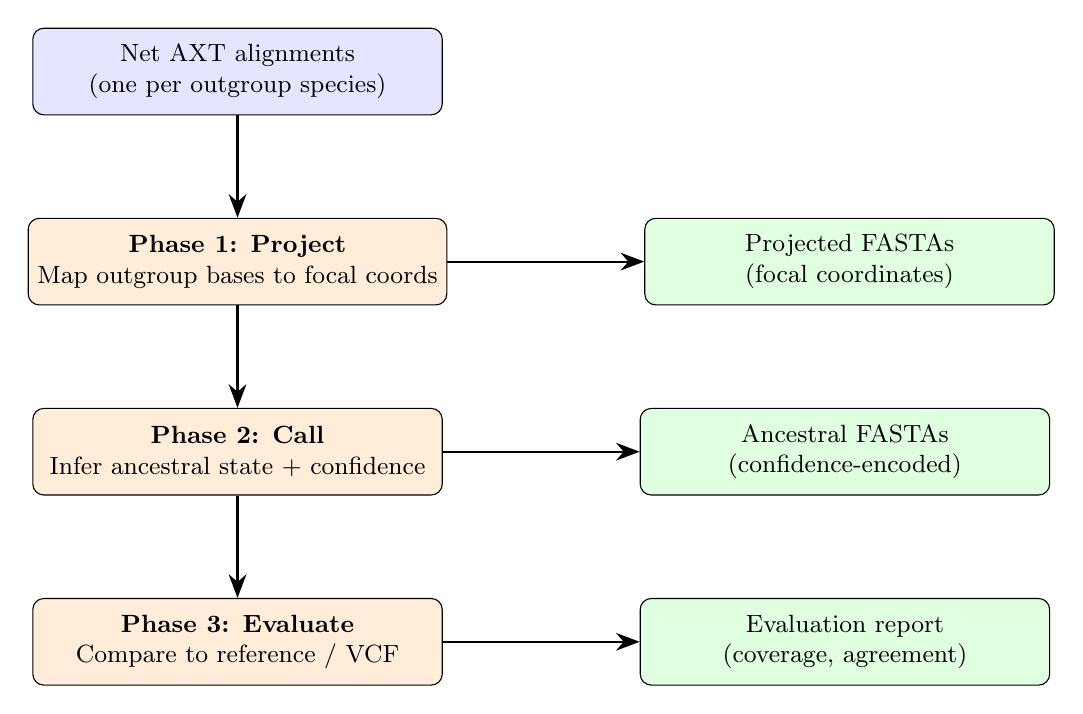
\begin{tikzpicture}[
    box/.style={draw, rounded corners, minimum width=5.2cm, minimum height=1.1cm,
                align=center, font=\small},
    arr/.style={-{Stealth[length=3mm]}, thick},
    node distance=1.3cm
]
\node[box, fill=blue!10] (input) {Net AXT alignments\\(one per outgroup species)};
\node[box, fill=orange!15, below=of input] (phase1) {\textbf{Phase 1: Project}\\Map outgroup bases to focal coords};
\node[box, fill=orange!15, below=of phase1] (phase2) {\textbf{Phase 2: Call}\\Infer ancestral state + confidence};
\node[box, fill=orange!15, below=of phase2] (phase3) {\textbf{Phase 3: Evaluate}\\Compare to reference / VCF};
\node[box, fill=green!12, right=2.5cm of phase1] (proj) {Projected FASTAs\\(focal coordinates)};
\node[box, fill=green!12, right=2.5cm of phase2] (anc) {Ancestral FASTAs\\(confidence-encoded)};
\node[box, fill=green!12, right=2.5cm of phase3] (eval) {Evaluation report\\(coverage, agreement)};

\draw[arr] (input) -- (phase1);
\draw[arr] (phase1) -- (phase2);
\draw[arr] (phase2) -- (phase3);
\draw[arr] (phase1) -- (proj);
\draw[arr] (phase2) -- (anc);
\draw[arr] (phase3) -- (eval);
\end{tikzpicture}
\caption{Overview of the ancify pipeline. Three sequential phases transform
raw pairwise alignments into confidence-encoded ancestral FASTA files. Phase~3
is optional.}
\label{fig:pipeline}
\end{figure}

All behavior is controlled by a single YAML configuration file that specifies
the focal species, outgroup species with their alignment files, inference
method, and optional evaluation parameters.

% ── 2.2 Phase 1: Coordinate Projection ──────────────────────────────────
\subsection{Phase~1: Coordinate projection}
\label{sec:projection}

The pipeline reads pairwise \emph{net} AXT alignment files from UCSC. These
represent best-in-genome, one-to-one alignments between the focal and each
outgroup species, produced by the netting algorithm that resolves overlapping
alignment chains by retaining only the highest-scoring chain at each position
\citep{Kent2003}.

Each AXT alignment block contains a header line with coordinates, followed by
the focal (target) and outgroup (query) sequences. For each block, the
projection algorithm maps outgroup bases onto the focal genome's coordinates:

\begin{itemize}
    \item If the focal position is a nucleotide, the corresponding outgroup
        base is recorded at that focal position.
    \item If the focal position is a gap character ($-$), the position is
        skipped (it represents an insertion in the outgroup with no
        corresponding focal coordinate).
    \item Positions not covered by any alignment block are filled with
        \texttt{N} (missing data).
\end{itemize}

The result is a FASTA file for each (outgroup, chromosome) pair with the same
length as the focal chromosome. The implementation uses a two-pass
architecture:

\begin{enumerate}
    \item \textbf{Parse pass:} Stream through the AXT file, collecting block
        metadata (start position, target sequence, query sequence) for the
        target chromosome.
    \item \textbf{Scatter pass:} Convert sequences to NumPy byte arrays and
        fill the output array using vectorized indexing operations.
\end{enumerate}

The scatter operation replaces the original per-character Python loop with a
vectorized NumPy operation. For each alignment block with focal sequence
$\mathbf{h}$ and outgroup sequence $\mathbf{c}$ starting at position $s$:

\begin{equation}
\label{eq:scatter}
\text{seq}[\text{pos}[j]] \leftarrow c_j \quad \forall\, j \text{ where } h_j \in \{A,C,G,T,N\}
\end{equation}

\noindent where $\text{pos}[j] = s - 1 + |\{k \le j : h_k \in \{A,C,G,T,N\}\}| - 1$
is the cumulative count of non-gap focal characters up to index $j$, mapped to
the 0-based focal coordinate.

% ── 2.3 Phase 2: Ancestral Calling ──────────────────────────────────────
\subsection{Phase~2: Ancestral state inference}
\label{sec:calling}

Phase~2 determines the ancestral allele at every genomic position. Three
inference methods are supported, sharing a common confidence-encoding scheme.

% ── 2.3.1 Two-Tier Voting ────────────────────────────────────────────────
\subsubsection{Method~1: Two-tier outgroup voting}
\label{sec:voting}

The default method partitions outgroup species into two phylogenetic tiers.
\emph{Inner} outgroups are closely related species whose sequences cover a
large fraction of the genome but may share derived alleles through ILS.
\emph{Outer} outgroups are more distantly related species that serve as an
independent evolutionary check.

At each position $i$, the algorithm proceeds as follows:

\begin{lstlisting}[caption={Two-tier outgroup voting (pseudocode).},
label={alg:voting},language={},numbers=none,frame=single,
basicstyle=\ttfamily\small]
Input:  Inner bases B_in, outer bases B_out,
        thresholds f_in, f_out
Output: Confidence-encoded ancestral character a_i

c_in  <- MajorityVote(B_in,  f_in)
c_out <- MajorityVote(B_out, f_out)

if c_in != N and c_in == c_out:
    return c_in              # High confidence (UPPERCASE)
elif c_in == N and c_out != N:
    return lower(c_out)      # Low confidence (lowercase)
elif c_in != N and c_out == N:
    return lower(c_in)       # Low confidence (lowercase)
elif c_in == N and c_out == N:
    return N                 # No data
else:
    return n                 # Disagreement (unresolved)
\end{lstlisting}

The \textsc{MajorityVote} function selects the most frequent nucleotide
among valid bases $\{A, C, G, T\}$, breaking ties alphabetically for
determinism ($A > C > G > T$). If no allele reaches the minimum frequency
threshold, the consensus is $N$ (missing).

The two-tier design guards against ILS: because the inner outgroups are
closely related, they are not independent observations---they may all share
a derived allele inherited from a polymorphic ancestral population. The outer
outgroup, being phylogenetically more distant, provides an independent check.
When both tiers agree, the call is high-confidence; when they disagree, the
position is flagged rather than erroneously resolved.

The \texttt{min\_inner\_freq} and \texttt{min\_outer\_freq} parameters
control a coverage--accuracy trade-off. With $k$ inner outgroups and
\texttt{min\_inner\_freq}$=m$, at least $m$ species must agree for a
consensus. Higher thresholds increase specificity at the cost of marking more
positions as missing.

% ── 2.3.2 Fitch Parsimony ───────────────────────────────────────────────
\subsubsection{Method~2: Fitch parsimony}
\label{sec:parsimony}

The second method applies the Fitch algorithm \citep{Fitch1971} to
reconstruct the most parsimonious ancestral state at the root of a
user-supplied phylogenetic tree. This method is preferred when the user has
three or more outgroups at varying phylogenetic distances and wants the tree
topology to determine how species are weighted.

The algorithm operates in two passes over the tree at each genomic position:

\begin{lstlisting}[caption={Fitch parsimony for ancestral state reconstruction
(pseudocode).},label={alg:fitch},language={},numbers=none,frame=single,
basicstyle=\ttfamily\small]
Input:  Rooted tree T, observed alleles {a_l} at leaves
Output: Root allele a_hat, ambiguity flag

--- Pass 1: Bottom-up (post-order) ---
for each leaf l:
    if a_l in {A, C, G, T}:
        S(l) <- {a_l}
    else:
        S(l) <- {A, C, G, T}     # Missing: wildcard

for each internal node v (post-order):
    if intersection of children's sets != empty:
        S(v) <- intersection of S(u) for u in children(v)
    else:
        S(v) <- union of S(u) for u in children(v)

--- Pass 2: Top-down (pre-order) ---
for each node v (pre-order, from root):
    if parent's allele in S(v):
        a_hat(v) <- parent's allele   # Minimize mutations
    else:
        a_hat(v) <- min(S(v))         # Alphabetical tie-break

a_hat    <- a_hat(root)
ambiguous <- |S(root)| > 1
\end{lstlisting}

The intersection step identifies alleles compatible with all children (no
mutation needed on those branches); the union step applies when at least one
mutation is required. Missing data at a leaf is handled by assigning the full
allele set $\{A,C,G,T\}$, making the leaf compatible with any state and
ensuring that missing data never forces unnecessary mutations.

The Newick tree is parsed by a recursive-descent parser that supports branch
lengths (parsed but unused by the Fitch algorithm) and both quoted and
unquoted labels.

\paragraph{Comparison with voting.}
Consider a position where bonobo$=$G, chimp$=$G, gorilla$=$A, macaque$=$A.
The voting method with inner$=\{\text{bonobo, chimp, gorilla}\}$ yields inner
consensus~G (majority 2:1), outer consensus~A, and flags the position as
unresolved ($n$). Fitch parsimony on the tree
\texttt{(((bonobo,chimp),gorilla),macaque)} infers root state~A with a single
G$\to$A mutation on the bonobo--chimp branch---a high-confidence call.

% ── 2.3.3 ML Classifier ─────────────────────────────────────────────────
\subsubsection{Method~3: Machine learning classifier}
\label{sec:ml}

The third method trains a LightGBM \citep{Ke2017} gradient-boosted
multi-class classifier (4~classes: A, C, G, T) to predict the ancestral
allele from a per-position feature vector. This approach can learn
substitution biases---such as elevated C$\to$T rates at CpG sites---and local
sequence context that the rule-based methods do not capture.

\paragraph{Feature engineering.}
For each genomic position, a feature vector of dimension $K + 9$ is
constructed from $K$ outgroup species (Table~\ref{tab:features}).

\begin{table}[t]
\centering
\caption{Per-position features for the ML classifier. $K$ denotes the total
number of outgroup species.}
\label{tab:features}
\begin{tabular}{@{}lp{7.5cm}c@{}}
\toprule
Feature & Description & Count \\
\midrule
Outgroup bases & Integer-encoded base per outgroup (0--3; $-1$ for missing) & $K$ \\
Data count & Number of outgroups with valid data & 1 \\
Agreement ratio & Fraction of valid outgroups agreeing with majority & 1 \\
Inner consensus & Majority base among inner outgroups (0--4) & 1 \\
Outer consensus & Majority base among outer outgroups (0--4) & 1 \\
Voting agreement & Whether inner $=$ outer (binary) & 1 \\
GC content & GC fraction in $\pm 50$\,bp window & 1 \\
CpG flag & Whether site is part of a CpG dinucleotide & 1 \\
Flanking bases & Bases immediately upstream and downstream & 2 \\
\bottomrule
\end{tabular}
\end{table}

The first $K$ features capture raw outgroup data. The next five features
encode the same information the voting method uses, enabling the model to
learn when voting is reliable. The final four context features capture
position-dependent substitution biases.

\paragraph{Training.}
Two label sources are supported:

\begin{enumerate}
    \item \textbf{Self-supervised:} Positions where the voting method's inner
        and outer tiers agree (uppercase output) serve as training labels. No
        external data is needed.
    \item \textbf{Reference-supervised:} An external ancestral reference
        (e.g., Ensembl EPO) provides ground-truth labels.
\end{enumerate}

Training subsamples up to $\sim$5~million sites per chromosome, stratified by
allele class to maintain class balance. The LightGBM model uses 200~boosting
iterations with 63~leaves per tree, learning rate~0.1, and 80\% feature and
bagging fractions.

\paragraph{Confidence calibration.}
The predicted class probability $p$ maps to confidence levels:

\begin{equation}
\label{eq:ml_conf}
a_i = \begin{cases}
    \text{uppercase}(c_i) & \text{if } p \ge \theta_\text{high} \\
    \text{lowercase}(c_i) & \text{if } \theta_\text{low} \le p < \theta_\text{high} \\
    n & \text{if } p < \theta_\text{low} \\
    N & \text{if all outgroups missing}
\end{cases}
\end{equation}

\noindent where $c_i$ is the predicted base and $\theta_\text{high} = 0.8$,
$\theta_\text{low} = 0.5$ by default. These thresholds can be tuned to trade
precision for recall.

% ── 2.4 Confidence Encoding ──────────────────────────────────────────────
\subsection{Confidence encoding}
\label{sec:confidence}

All three methods produce output in a unified FASTA format where letter case
encodes confidence (Table~\ref{tab:confidence}). This convention is compatible
with the Ensembl EPO ancestral sequence format, allowing seamless integration
with existing workflows.

\begin{table}[t]
\centering
\caption{Confidence encoding scheme shared by all inference methods.
Typical fractions are for human autosomes with the BCGM outgroup
configuration.}
\label{tab:confidence}
\begin{tabular}{@{}llll@{}}
\toprule
Character & Confidence & Condition & Typical fraction \\
\midrule
\texttt{ACGT} & High & Both tiers agree / unambiguous parsimony / $p \ge 0.8$ & $\sim$75\% \\
\texttt{acgt} & Low & One tier only / ambiguous parsimony / $0.5 \le p < 0.8$ & $\sim$15\% \\
\texttt{n} & Unresolved & Tiers disagree / $p < 0.5$ & $\sim$0.1\% \\
\texttt{N} & Missing & No data from either tier / all outgroups missing & $\sim$10\% \\
\bottomrule
\end{tabular}
\end{table}

This encoding means that a single FASTA file carries both the ancestral call
and its reliability, eliminating the need for sidecar quality files. Downstream
analyses can select their stringency: conservative analyses use only uppercase
positions, while maximum-coverage analyses include lowercase calls.

% ══════════════════════════════════════════════════════════════════════════
\section{Implementation}
\label{sec:implementation}

% ── 3.1 Software Architecture ────────────────────────────────────────────
\subsection{Software architecture}
\label{sec:architecture}

ancify is implemented in Python ($\ge$3.8) and organized as a modular
package (Figure~\ref{fig:architecture}). Core dependencies are limited to
PyYAML and NumPy; optional dependencies include PyTorch (GPU acceleration),
LightGBM (ML method), \texttt{isal} (faster gzip I/O), and
\texttt{scikit-allel} (VCF evaluation).

\begin{figure}[t]
\centering
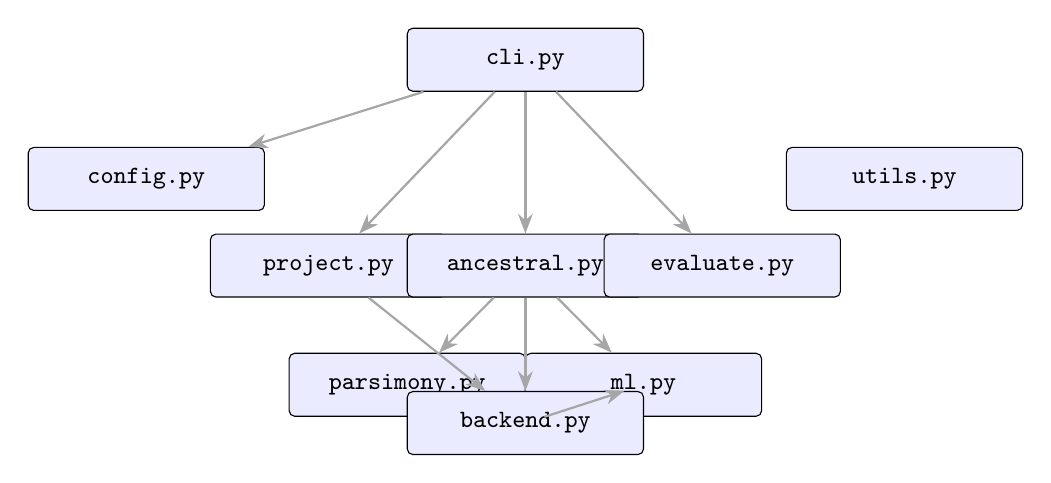
\begin{tikzpicture}[
    mod/.style={draw, rounded corners=2pt, minimum width=3cm, minimum height=0.8cm,
                align=center, font=\small\ttfamily, fill=blue!8},
    arr/.style={-{Stealth[length=2.5mm]}, thick, gray!70},
    node distance=0.7cm and 1.8cm
]
\node[mod] (cli) {cli.py};
\node[mod, below left=of cli] (config) {config.py};
\node[mod, below right=of cli] (utils) {utils.py};
\node[mod, below=1.8cm of cli, xshift=-2.5cm] (project) {project.py};
\node[mod, below=1.8cm of cli] (ancestral) {ancestral.py};
\node[mod, below=1.8cm of cli, xshift=2.5cm] (evaluate) {evaluate.py};
\node[mod, below=of ancestral, xshift=-1.5cm] (parsimony) {parsimony.py};
\node[mod, below=of ancestral, xshift=1.5cm] (ml) {ml.py};
\node[mod, below=3.8cm of cli] (backend) {backend.py};

\draw[arr] (cli) -- (config);
\draw[arr] (cli) -- (project);
\draw[arr] (cli) -- (ancestral);
\draw[arr] (cli) -- (evaluate);
\draw[arr] (ancestral) -- (parsimony);
\draw[arr] (ancestral) -- (ml);
\draw[arr] (project) -- (backend);
\draw[arr] (ancestral) -- (backend);
\draw[arr] (ml) -- (backend);
\end{tikzpicture}
\caption{Module dependency graph of the ancify package. The \texttt{backend}
module abstracts CPU (NumPy) and GPU (PyTorch) execution.}
\label{fig:architecture}
\end{figure}

\begin{description}[style=nextline,leftmargin=1em]
    \item[\texttt{cli.py}] Command-line interface with subcommands
        \texttt{init}, \texttt{project}, \texttt{call}, \texttt{evaluate},
        \texttt{run}, and \texttt{train}.
    \item[\texttt{config.py}] YAML configuration loading, validation, and
        dataclass-based representation (\texttt{PipelineConfig},
        \texttt{OutgroupSpec}, \texttt{EvaluationConfig}).
    \item[\texttt{project.py}] Phase~1: two-pass AXT parsing and vectorized
        scatter-based coordinate projection.
    \item[\texttt{ancestral.py}] Phase~2: dispatches to voting, parsimony,
        or ML calling with parallel execution across chromosomes.
    \item[\texttt{parsimony.py}] Fitch algorithm implementation: tree data
        structure (\texttt{TreeNode}), recursive-descent Newick parser,
        bottom-up and top-down traversals.
    \item[\texttt{ml.py}] Feature extraction, LightGBM training, prediction,
        and confidence encoding.
    \item[\texttt{evaluate.py}] Phase~3: coverage statistics, reference
        comparison, and VCF concordance.
    \item[\texttt{utils.py}] FASTA I/O (handles gzip transparently),
        chromosome lengths parsing, and the scalar majority vote function.
    \item[\texttt{backend.py}] CPU/GPU backend abstraction: auto-detection,
        sequence encoding, vectorized majority vote, vectorized ancestral
        calling, and vectorized block scatter.
\end{description}

% ── 3.2 GPU Acceleration ─────────────────────────────────────────────────
\subsection{GPU acceleration}
\label{sec:gpu}

The backend module provides transparent GPU acceleration through PyTorch
tensor operations. Sequences are encoded as \texttt{uint8} arrays
($A=0, C=1, G=2, T=3$; all else$=4$). The vectorized majority vote replaces
per-position Python calls with column-wise tensor operations over the
entire chromosome:

\begin{equation}
\label{eq:gpu_vote}
\text{counts}[b, :] = \sum_{s=1}^{K} \mathbb{1}\left[\text{encoded}[s, :] = b\right], \quad b \in \{0,1,2,3\}
\end{equation}

\begin{equation}
\label{eq:gpu_winner}
\text{winner}[:] = \arg\max_{b} \text{counts}[b, :], \quad
\text{winner}[j] = 4 \;\text{if}\; \max_b \text{counts}[b, j] < f_\text{min}
\end{equation}

The confidence assignment uses approximately 15~tensor operations for an
entire chromosome, replacing 248~million Python function calls for human
chr1. The encoding of bases as consecutive integers 0--3 ensures that
\texttt{torch.max(dim=0)} returns the first index among tied maxima,
reproducing the alphabetical tie-breaking of the scalar implementation.
All code paths produce bit-identical output, verified by the test suite.

Multi-GPU processing distributes chromosomes across available CUDA devices
in round-robin fashion. Memory requirements are modest: approximately 6\,GB
per chromosome for human chr1 with four outgroups, fitting comfortably on
consumer GPUs with 8--12\,GB VRAM.

Table~\ref{tab:performance} summarizes the performance characteristics.

\begin{table}[t]
\centering
\caption{Wall-clock time for the full human genome (hg38, 4~outgroups) under
different backends. GPU timings are for a single NVIDIA A100.}
\label{tab:performance}
\begin{tabular}{@{}llll@{}}
\toprule
Component & Scalar Python & Vectorized CPU & GPU (PyTorch) \\
\midrule
Phase 1 (projection) & $\sim$4 hours & $\sim$5 minutes & $\sim$2 minutes \\
Phase 2 (calling) & $\sim$8 hours & $\sim$10 minutes & $\sim$10 seconds \\
\midrule
\textbf{Total} & $\sim$12 hours & $\sim$15 minutes & $\sim$2 minutes \\
\bottomrule
\end{tabular}
\end{table}

% ── 3.3 Configuration System ─────────────────────────────────────────────
\subsection{Configuration system}
\label{sec:config}

All pipeline behavior is controlled by a single YAML configuration file.
A minimal configuration specifies the focal species label, a chromosome
lengths file, the outgroup species with their alignment files, and an output
directory. Listing~\ref{lst:config} shows a typical configuration for human
ancestral allele calling.

\begin{lstlisting}[language=yaml,caption={Minimal YAML configuration for
human (hg38) ancestral calling with four outgroups.},
label={lst:config}]
focal_species: human
chromosome_lengths: chromoLens.txt

outgroups:
  inner:
    - name: bonobo
      alignment: hg38.panPan3.net.axt.gz
    - name: chimp
      alignment: hg38.panTro6.net.axt.gz
    - name: gorilla
      alignment: hg38.gorGor6.net.axt.gz
  outer:
    - name: macaque
      alignment: hg38.rheMac10.net.axt.gz

output_dir: ./ancestral_calls
num_cpus: 24
\end{lstlisting}

Optional fields include \texttt{method} (\texttt{"voting"},
\texttt{"parsimony"}, or \texttt{"ml"}), \texttt{tree} (Newick string or
file path), \texttt{backend} (\texttt{"auto"}, \texttt{"cpu"}, or
\texttt{"gpu"}), \texttt{gpu\_devices}, frequency thresholds, and an
\texttt{evaluation} block for Phase~3.

% ── 3.4 Species Agnosticism ──────────────────────────────────────────────
\subsection{Species agnosticism}
\label{sec:species}

ancify is not restricted to any particular organism. It operates on standard
AXT alignment files that are available from the UCSC Genome Browser for
hundreds of species pairs. Table~\ref{tab:species} shows example
configurations for several model and non-model organisms.

\begin{table}[t]
\centering
\caption{Example outgroup configurations for different focal species.
Divergence times are approximate.}
\label{tab:species}
\begin{tabular}{@{}llll@{}}
\toprule
Focal species & Inner outgroups & Outer outgroup & Divergence \\
\midrule
Human & Bonobo, Chimp, Gorilla & Macaque & 6--25\,Mya \\
Mouse & Rat & Rabbit & 12--90\,Mya \\
\textit{D.~melanogaster} & \textit{D.~simulans}, \textit{D.~sechellia} & \textit{D.~yakuba} & 2.5--6\,Mya \\
\textit{Brassica rapa} & \textit{B.~oleracea} & \textit{A.~thaliana} & 20\,Mya \\
Zebrafish & Medaka & Fugu & --- \\
\bottomrule
\end{tabular}
\end{table}

% ══════════════════════════════════════════════════════════════════════════
\section{Validation}
\label{sec:validation}

% ── 4.1 Reference Comparison ─────────────────────────────────────────────
\subsection{Comparison with Ensembl EPO}
\label{sec:epo}

The BCGM (bonobo + chimp + gorilla + macaque) calling method was validated
against the Ensembl EPO 13-primate ancestral reference for human GRCh38.
Table~\ref{tab:validation} summarizes the results.

\begin{table}[t]
\centering
\caption{Validation of ancify BCGM calls against the Ensembl EPO 13-primate
ancestral reference and 1000~Genomes Phase~3 VCFs. Coverage is defined as the
fraction of positions with a non-\texttt{N} ancestral call.}
\label{tab:validation}
\begin{tabular}{@{}lrrr@{}}
\toprule
Metric & chr1 & chr22 & chrX \\
\midrule
Coverage (ancify BCGM) & 79.1\% & 74.6\% & 44.4\% \\
Coverage (Ensembl EPO) & 90.2\% & 81.2\% & 44.1\% \\
Disagreement rate & 0.08\% & 0.11\% & 3.51\% \\
Matches REF or ALT (VCF) & 99.6\% & 99.5\% & 99.3\% \\
\bottomrule
\end{tabular}
\end{table}

Autosomal chromosomes exhibit excellent agreement with the EPO reference,
with disagreement rates below 0.12\%. The higher disagreement on chrX
(3.51\%) reflects the reduced effective population size and male
hemizygosity, which increase ILS rates in the human--great ape clade.

The coverage difference between ancify (79.1\% on chr1) and EPO (90.2\%)
is expected: ancify uses 4~species whereas EPO uses 13, providing greater
alignment coverage. Including low-confidence (lowercase) positions raises
ancify's coverage from approximately 79\% to approximately 90\% on chr1.

% ── 4.2 VCF Concordance ─────────────────────────────────────────────────
\subsection{VCF concordance}
\label{sec:vcf}

At known variant sites from the 1000~Genomes Project, the ancestral call
matches either the REF or ALT allele in $>$99.5\% of cases. The
approximately 95\% REF-matching fraction is expected, as reference genome
assemblies are constructed from common alleles that are typically ancestral.
The approximately 5\% ALT-matching fraction identifies sites where the
reference carries a derived allele---precisely the sites where polarization
provides the most value.

The $\sim$0.5\% of sites matching neither REF nor ALT are attributable to
triallelic sites (where both REF and ALT are derived and the true ancestral
allele is a third base), multi-allelic VCF records, and rare calling errors.

% ── 4.3 Evaluation Module ───────────────────────────────────────────────
\subsection{Built-in evaluation}
\label{sec:evalmodule}

Phase~3 computes three categories of metrics:

\begin{enumerate}
    \item \textbf{Coverage statistics:} The fraction of positions at each
        confidence level (high, low, unresolved, missing).
    \item \textbf{Reference comparison:} Position-by-position agreement and
        disagreement rates against an external ancestral reference.
    \item \textbf{VCF comparison:} The fraction of variant sites where the
        ancestral call matches REF, ALT, or neither.
\end{enumerate}

Results are written as structured text files in
\texttt{<output\_dir>/evaluation/}, one per chromosome.

% ══════════════════════════════════════════════════════════════════════════
\section{Usage}
\label{sec:usage}

% ── 5.1 Installation ─────────────────────────────────────────────────────
\subsection{Installation}

\begin{lstlisting}[language=bash,numbers=none]
pip install .                  # core (CPU)
pip install '.[evaluate]'      # + evaluation dependencies
pip install '.[fast]'          # + faster gzip (isal)
pip install '.[ml]'            # + LightGBM, scikit-learn

# GPU acceleration (PyTorch with CUDA)
pip install torch --index-url https://download.pytorch.org/whl/cu128
\end{lstlisting}

% ── 5.2 Command-Line Interface ───────────────────────────────────────────
\subsection{Command-line interface}

The pipeline is invoked through the \texttt{ancify} command:

\begin{lstlisting}[language=bash,numbers=none]
ancify init     [-o FILE]           # Generate template config
ancify project  -c CONFIG [-n N]    # Phase 1: project alignments
ancify call     -c CONFIG [-n N]    # Phase 2: call ancestral states
ancify evaluate -c CONFIG [-n N]    # Phase 3: evaluate (optional)
ancify run      -c CONFIG [-n N]    # All phases end-to-end
ancify train    -c CONFIG [-o MODEL]# Train ML model
\end{lstlisting}

Alternatively: \texttt{python -m ancify run -c config.yaml}.

% ── 5.3 Python API ───────────────────────────────────────────────────────
\subsection{Python API}

For programmatic use, all pipeline functions are importable:

\begin{lstlisting}[language=Python,caption={Programmatic usage of the ancify
Python API.},label={lst:api}]
from ancify.config import load_config
from ancify.project import run_projection
from ancify.ancestral import run_ancestral_calling
from ancify.ancestral import call_ancestral_base

# Full pipeline
cfg = load_config("config.yaml")
run_projection(cfg)
run_ancestral_calling(cfg)

# Single-position call
base = call_ancestral_base(
    inner_bases=["A", "A", "G"],
    outer_bases=["A"],
)  # Returns "A" (high confidence)
\end{lstlisting}

% ── 5.4 Downstream Integration ───────────────────────────────────────────
\subsection{Downstream integration}

The output ancestral FASTA files integrate directly into standard population
genetics workflows:

\begin{lstlisting}[language=Python,caption={Polarizing a VCF using ancify
output.},label={lst:polarize}]
from ancify.utils import read_fasta

_, seq = read_fasta("ancestral_calls/chr1.fa")

for variant in vcf:
    anc = seq[variant.POS - 1].upper()
    if anc == variant.REF:
        pass  # REF is ancestral
    elif anc == variant.ALT:
        pass  # ALT is ancestral (flip frequencies)
\end{lstlisting}

% ══════════════════════════════════════════════════════════════════════════
\section{Discussion}
\label{sec:discussion}

\subsection{Design philosophy}

ancify was designed with three priorities. First, \emph{simplicity}: a single
YAML file controls all behavior, and the pipeline reads standard file formats
available for hundreds of species. Second, \emph{transparency}: the
case-encoding of confidence levels enables users to make informed decisions
about which positions to trust without requiring auxiliary files or
probabilistic models. Third, \emph{performance}: the GPU backend makes
genome-wide analysis feasible in minutes rather than hours, enabling rapid
iteration during method development or when processing multiple species.

\subsection{Comparison of inference methods}

The three methods offer complementary strengths. The two-tier voting method
is the simplest, requiring no phylogenetic tree and making minimal assumptions
beyond the inner/outer partition. It is well-suited for the common case of
3--4 outgroups with a clear phylogenetic structure.

Fitch parsimony is more principled when the outgroup phylogeny is known,
as it accounts for the tree topology rather than treating species as
exchangeable within tiers. It resolves many positions that voting marks as
unresolved---particularly ILS-affected sites where the tree structure
disambiguates the ancestral state.

The ML classifier is most powerful when training data is available (either
self-supervised from high-confidence voting sites or reference-supervised
from an external ancestral sequence). It can learn substitution biases,
CpG effects, and local sequence context, and provides calibrated probability
scores rather than binary confidence levels. However, it requires an
additional training step and may overfit to biases present in the training
data.

\subsection{Limitations}

Several limitations should be noted:

\begin{enumerate}
    \item \textbf{Alignment dependence.} The accuracy of all methods is
        bounded by the quality of the input alignments. Regions with
        segmental duplications, recent transposable element insertions, or
        structural variants may produce incorrect projections.
    \item \textbf{No substitution model.} The voting and parsimony methods
        do not account for branch-length-weighted substitution probabilities.
        More sophisticated probabilistic methods (e.g., maximum likelihood
        on a substitution model) could improve accuracy at the cost of
        additional complexity.
    \item \textbf{Coverage limited by outgroup count.} With only 4~species,
        ancify's coverage (79\% high-confidence on human chr1) is lower than
        EPO's (90\%), which uses 13~species. Adding more outgroups would
        improve coverage.
    \item \textbf{ILS on the X chromosome.} The elevated disagreement rate
        on chrX (3.51\% vs.\ $<$0.12\% on autosomes) reflects genuine
        biological challenges that would require more outgroups or
        probabilistic modeling to address.
\end{enumerate}

\subsection{Future directions}

Planned extensions include support for probabilistic ancestral reconstruction
using continuous-time Markov models on the phylogenetic tree, integration with
\texttt{hal} format whole-genome alignments, and automated outgroup selection
based on alignment coverage and phylogenetic distance.

% ══════════════════════════════════════════════════════════════════════════
\section{Availability}
\label{sec:availability}

ancify is released under the MIT license. Source code, documentation, and
example configurations are available at:

\begin{center}
\url{https://github.com/kevinkorfmann/ancify}
\end{center}

\noindent Full documentation including tutorials, algorithm deep dives, and a
species adaptation guide is hosted at
\url{https://ancify.readthedocs.io}.

% ══════════════════════════════════════════════════════════════════════════
\section*{Acknowledgments}

The UCSC Genome Browser group is acknowledged for providing the pairwise
alignment infrastructure that makes this pipeline possible. The Ensembl
project is acknowledged for the EPO ancestral reference used in validation.

% ══════════════════════════════════════════════════════════════════════════
\bibliographystyle{plainnat}
\bibliography{references}

\end{document}
